\documentclass[10pt,aspectratio=149]{beamer}
\usecolortheme{Calm}
\usetheme{Calm}
%\usefonttheme[onlymath]{serif} % beamer force les maths en cmss par défaut, qui n'a pas de vrai gras : \mathbf{} restait fin
\usepackage{amsmath}
\usepackage{pgfplots}
\pgfplotsset{compat=1.18}
\usepackage{pgfplotstable}
\usepackage[utf8]{inputenc}
\usepackage{hyperref}
\RequirePackage[absolute,overlay]{textpos}
%\usepackage[sfdefault]{cabin}
%\usepackage[T1]{fontenc}
%\setlength{\TPHo{}rizModule}{\paperwidth}
%\setlength{\TPVertModule}{\paperheight}
%\definecolor{OQEdarkblue}{HTML}{046085}


\defbeamertemplate*{background canvas}{bg}
{%
  \color{lightgray!40}\vrule width\paperwidth height\paperheight% added bg color
}

% Centered, larger display equation
\newcommand{\keyeq}[1]{%
  \begin{center}
    \Large$\displaystyle #1$
  \end{center}%
}

% Same style, for a system of equations aligned on "="
% (rows separated by \\, each row written as LHS &= RHS)
\newcommand{\keyeqs}[1]{%
  \begin{center}
    \normalsize$\displaystyle
    \begin{aligned}
    #1
    \end{aligned}
    $
  \end{center}%
}

%------------------------------

\author{Dominique Gravel}
\title{Spatial cascades in metaecosystems}
\date{August 28th, 2026}
\institute{Université de Sherbrooke \\ Summer school in biodiversity modelling}

%------------------------------
% TITLE SLIDE
%------------------------------

\usebackgroundtemplate
{
  
\includegraphics[width=\paperwidth,height=\paperheight]{bg}%
}

\begin{document}

	\begin{frame}[plain]
		\titlepage
	\end{frame}

%------------------------------
% INTRO
%------------------------------

\begin{frame}{Island secondary productivity}
	
	\begin{center}
		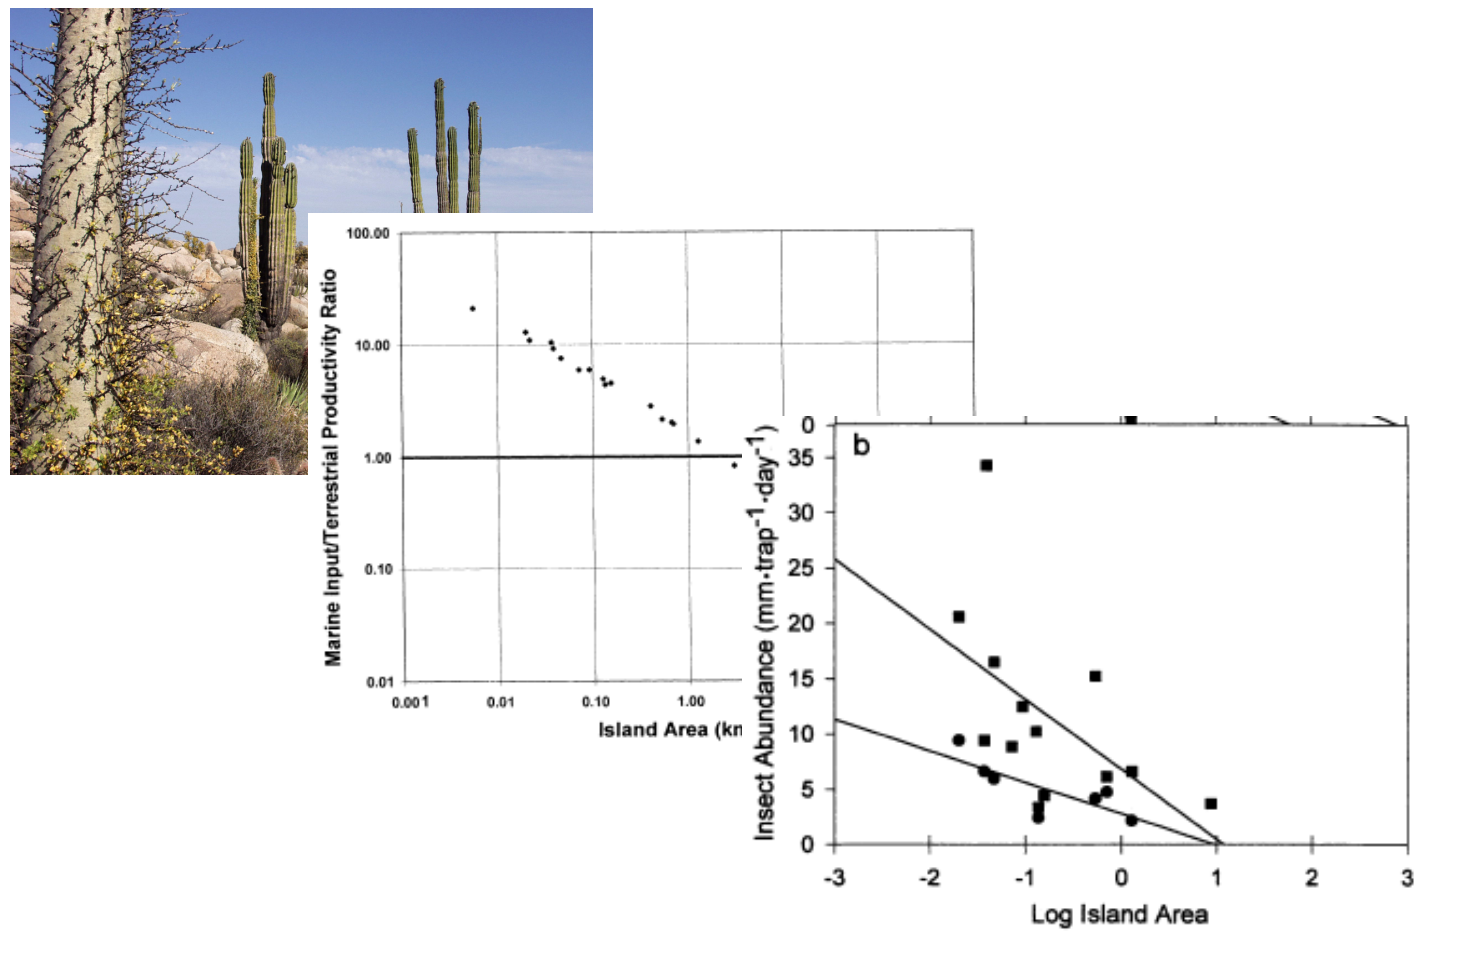
\includegraphics[height=0.8\textheight]{Figs/polis1995}\\
		\footnotesize Polis et Hurd. 1995, 1996
	\end{center}  

\end{frame}

%------------------------------

\begin{frame}{Apparent competition in the arctic}
	
	\begin{center}
		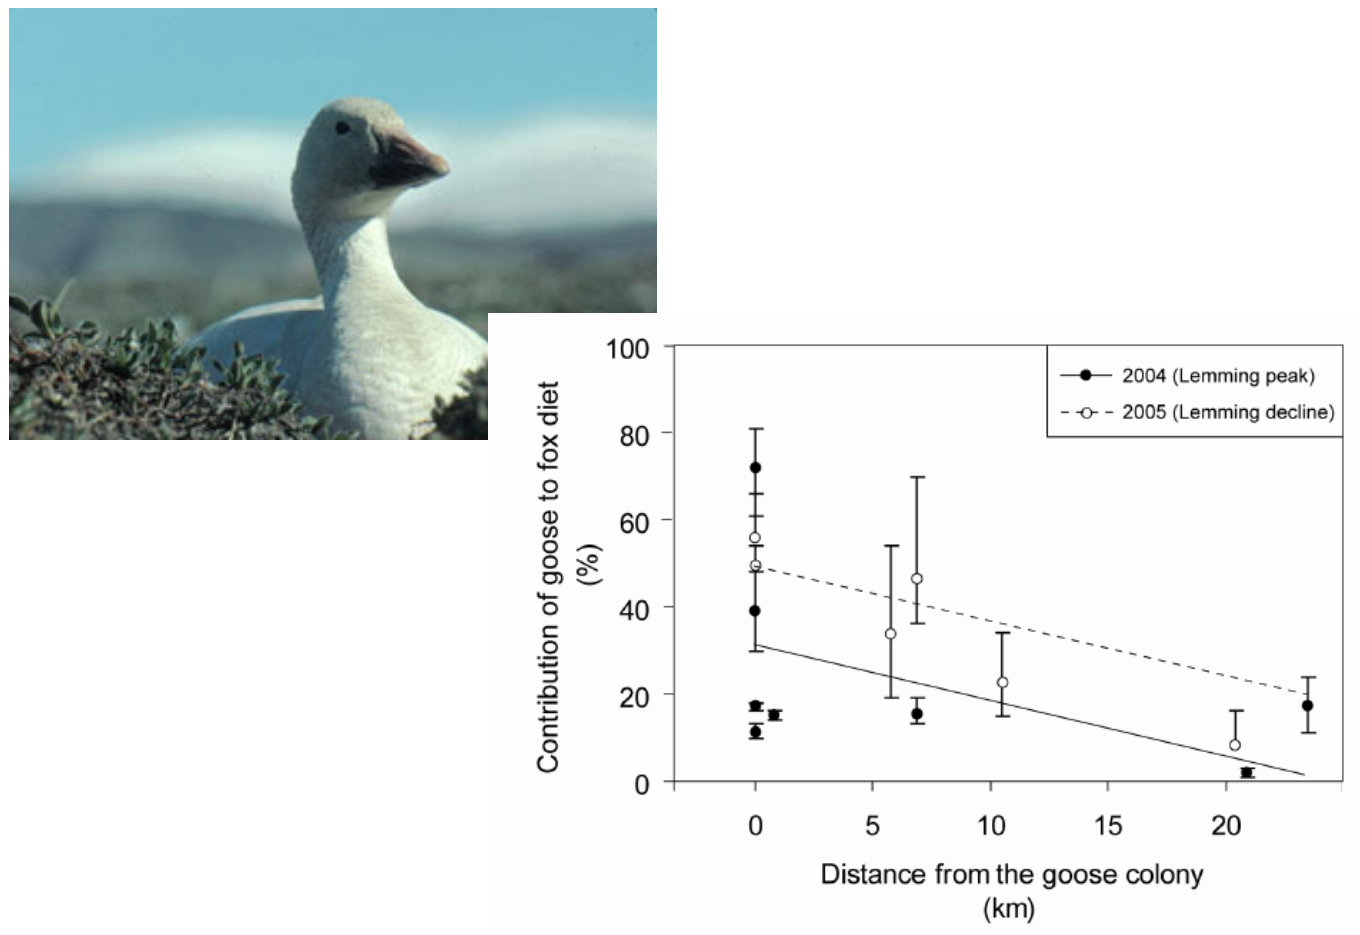
\includegraphics[height=0.7\textheight]{Figs/giroux2007}\\
		\footnotesize Giroux et al. 2007. JAE.
	\end{center}

\end{frame}

%------------------------------

\begin{frame}{Stream-forest interface}
	
	\begin{center}
		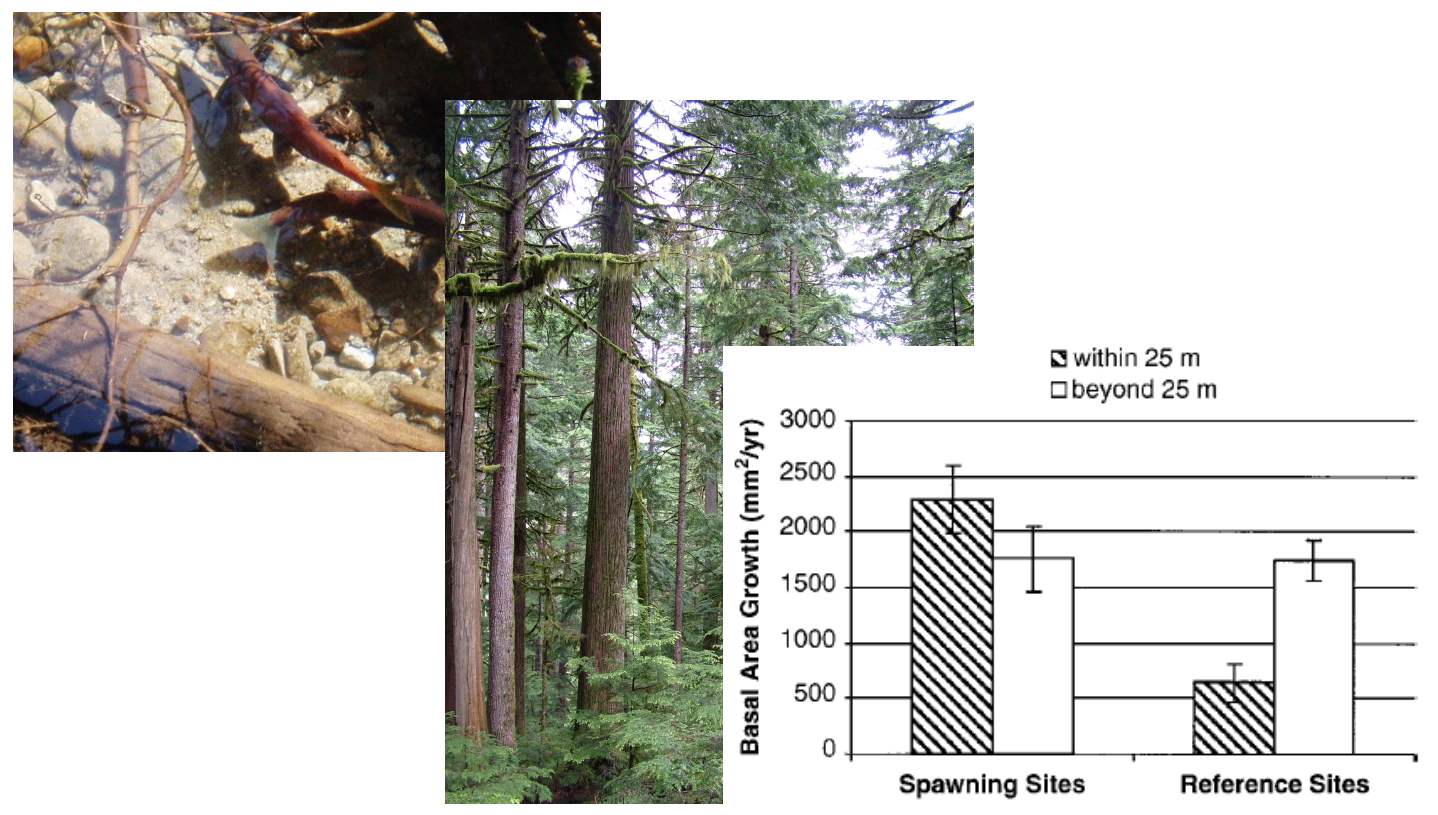
\includegraphics[height=0.7\textheight]{Figs/heldfield2001}\\
		\footnotesize Helfield and Naimoan. 2001.
	\end{center}

\end{frame}

%------------------------------

\begin{frame}{Seabirds colonies}
	
	\begin{center}
		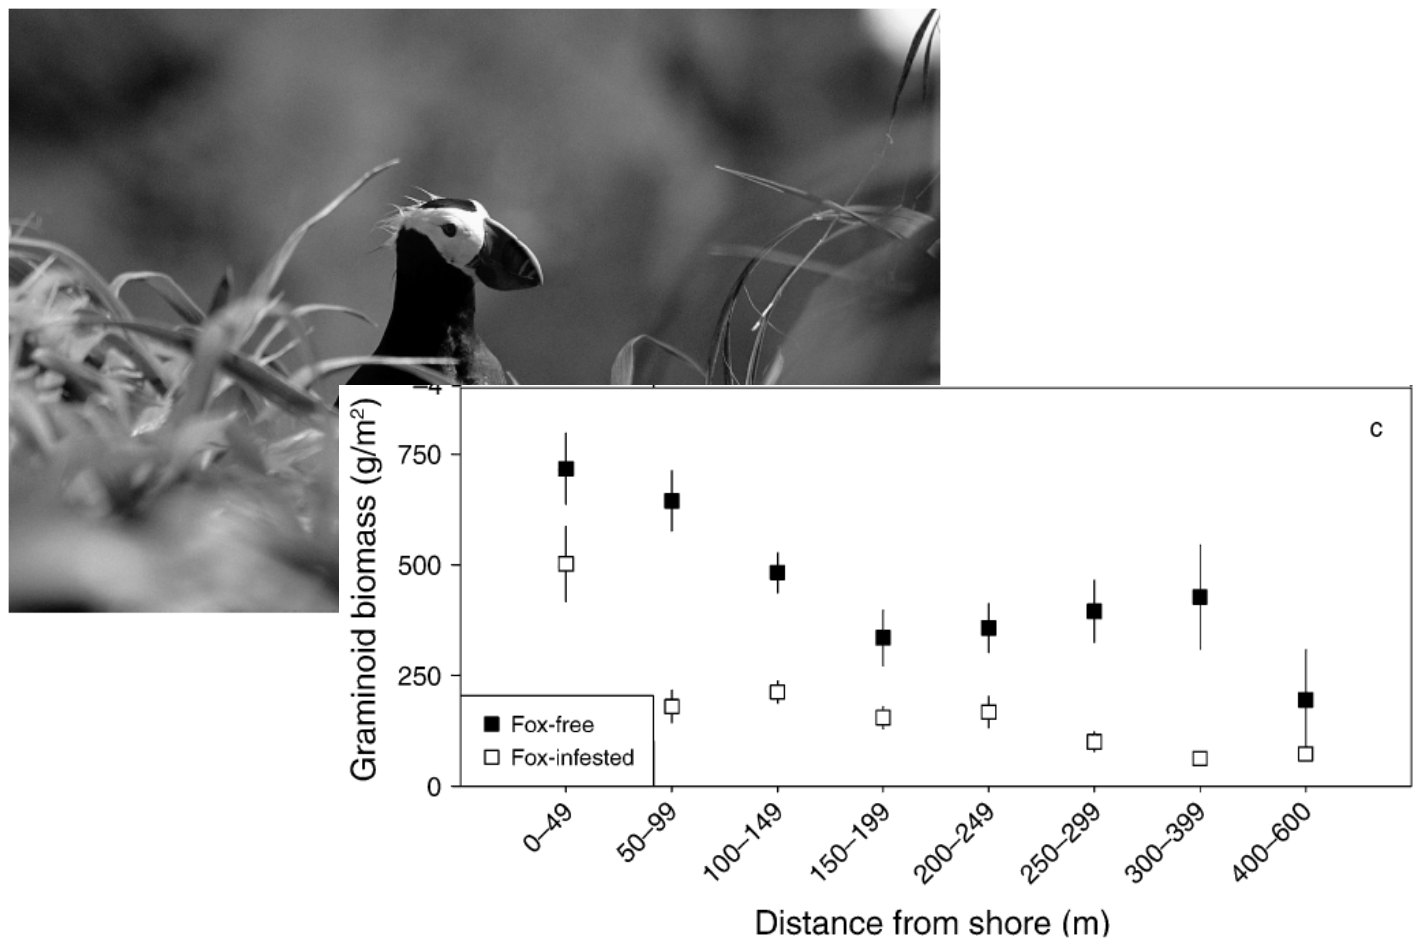
\includegraphics[height=0.7\textheight]{Figs/maron2006}\\
		\footnotesize Maron et al. 2006. Ecol. Monogr.
	\end{center}

\end{frame}

%------------------------------

\begin{frame}{Carbon fluxes}{Global scale}
	
	\begin{center}
		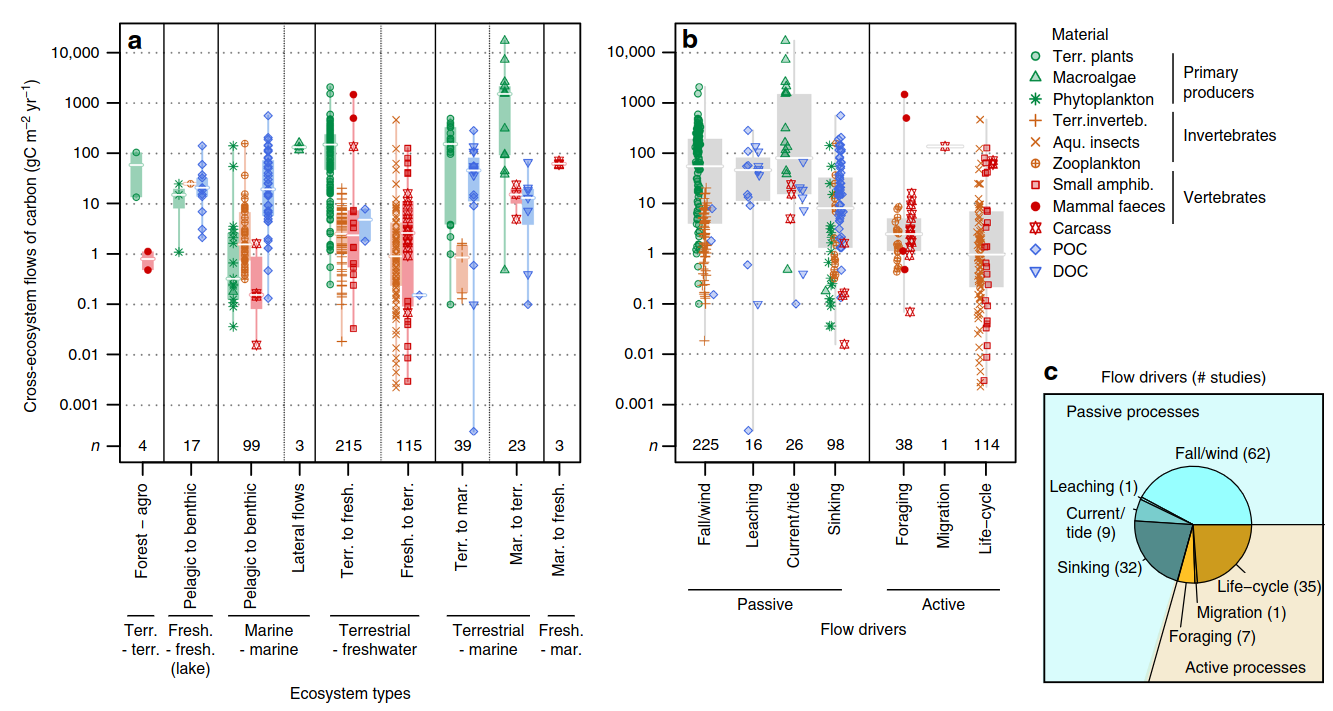
\includegraphics[height=0.7\textheight]{Figs/gounand2016}\\
		\footnotesize Gounand et al. 2016. Nat. Communications
	\end{center}

\end{frame}

%------------------------------

\begin{frame}{Spatial cascades}
	
	\begin{center}
		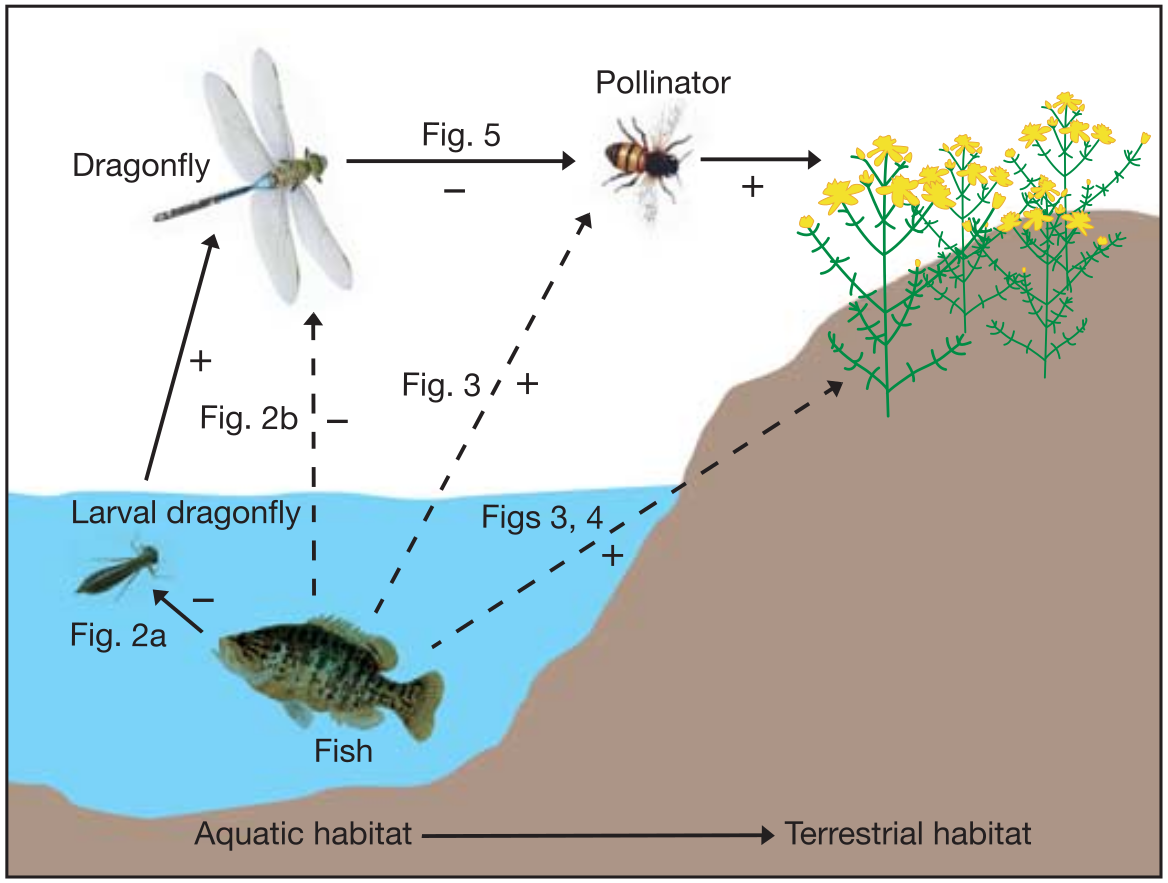
\includegraphics[height=0.7\textheight]{Figs/knight2005}\\
		\footnotesize Knight et al. 2005. Nature.
	\end{center}

\end{frame}

%------------------------------
% EXERCISE
%------------------------------

{
	\usebackgroundtemplate{}
	\begin{frame}
	
		\pagecolor{BDQC1st}
		\color{white}
	
		\LARGE{\textit{Exercise}}
	
	\end{frame}
}
		
%------------------------------
		
\begin{frame}{A minimal ecosystem model}{Two patches}
	
	\begin{center}
		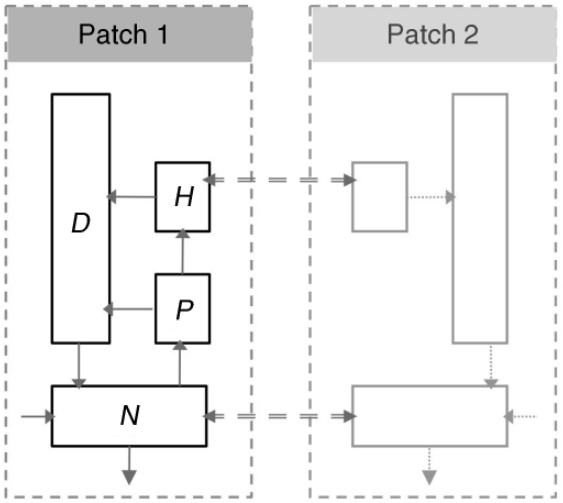
\includegraphics[height=0.7\textheight]{Figs/gravel2010a}\\
	\end{center}

\end{frame}

%------------------------------
		
\begin{frame}{A minimal ecosystem model}{Equations}
	
	\keyeqs{
		\frac{dN_x}{dt}
		= I_x + rD_x - e_NN_x - a_PN_xP_x
		+ d_N\left(N_{x+1} - N_x\right)
	}
	
	\keyeqs{
		\frac{dP_x}{dt}
		= a_PN_xP_x - m_PP_x - e_PP_x - a_HP_xH_x
		+ d_P\left(P_{x+1} - P_x\right)
	}
	
	\keyeqs{
		\frac{dH_x}{dt}
		= a_HP_xH_x - m_HH_x - e_HH_x
		+ d_H\left(H_{x+1} - H_x\right)
	}
	
	\keyeqs{
		\frac{dD_x}{dt}
		= m_PP_x + m_HH_x - (r + e_D)D_x
		+ d_D\left(D_{x+1} - D_x\right)
	}

\end{frame}

%------------------------------
		
\begin{frame}{Exercise}
	
	\begin{itemize}
		\item Consider a chain of lakes connected by streams
		\item Starting with plants and detritus only, look at the distribution of stocks from one location to another 		
		\item Add herbivores, how is it changing ?
		\item Decrease progressively the external input $I_x$, what is happening ?
	\end{itemize}
	
\end{frame}

%------------------------------

{
	\usebackgroundtemplate{}
	\begin{frame}
	
		\pagecolor{BDQC1st}
		\color{white}
	
		\LARGE{\textit{Source and sink dynamics in metaecosystems}}
	
	\end{frame}
}
		
%------------------------------
% SOURCE-SINK THEORY
%------------------------------
				
\begin{frame}{Metaecosystems}
	
	\textbf{Definition} : a set of ecosystems connected by spatial flows of energy, materials and organisms across ecosystem boundaries (Loreau et al. 2003, Eco Lett.)
	
	\textit{Less appreciated is the fact that these flows may also impose global constraints at the scale of the meta-ecosystem as a whole, thereby generating a strong interdependence among local ecosystems. [] which means that some compartments must be sources whereas others must be sinks in each ecosystem}

\end{frame}

%------------------------------
		
\begin{frame}{Direction of spatial flows}
	
	\begin{center}
		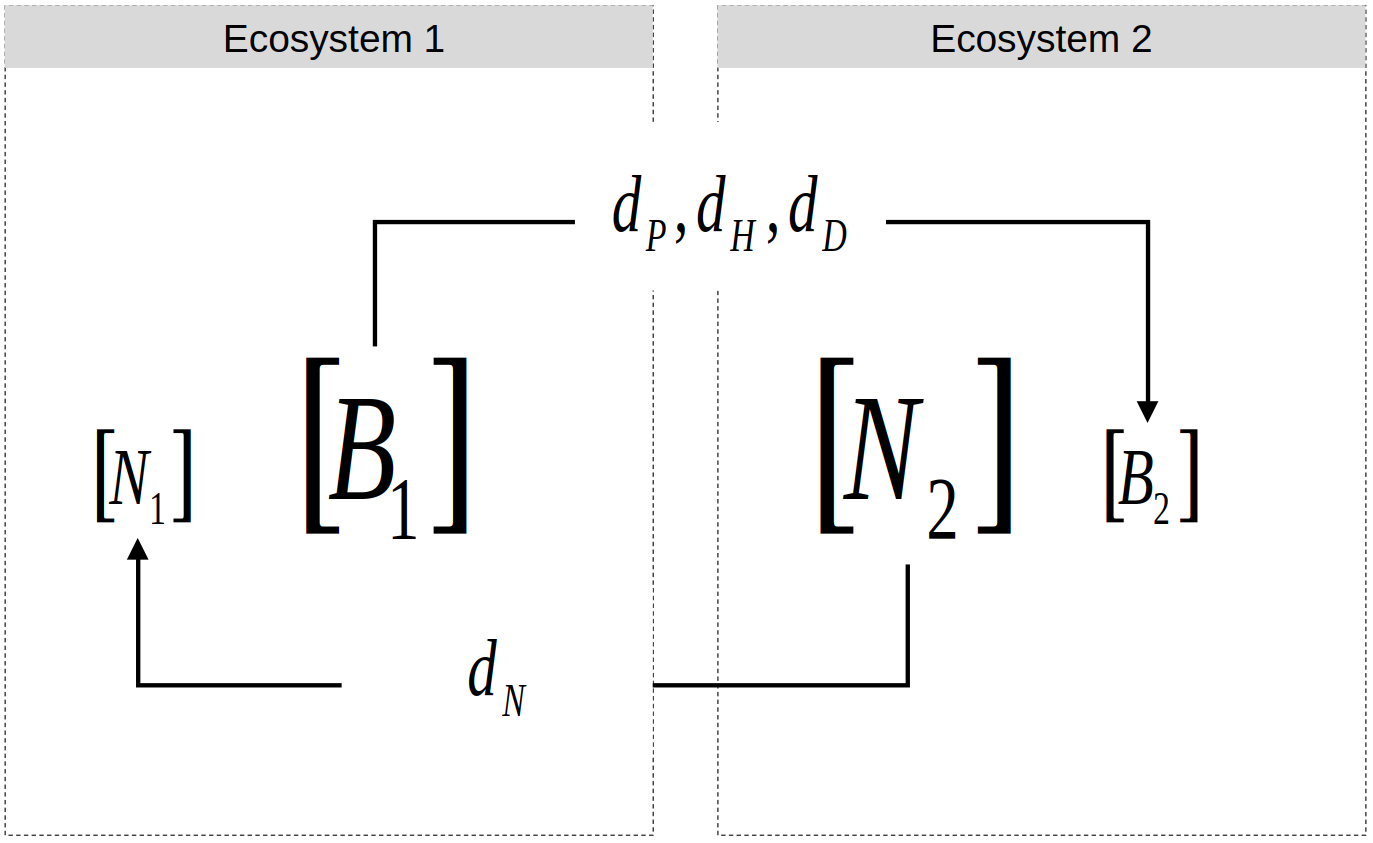
\includegraphics[height=0.7\textheight]{Figs/gravel2010b}\\
		\footnotesize Gravel et al. 2010. Ecology
	\end{center}

\end{frame}

%------------------------------
		
\begin{frame}{Primary productivity}
	
	\begin{center}
		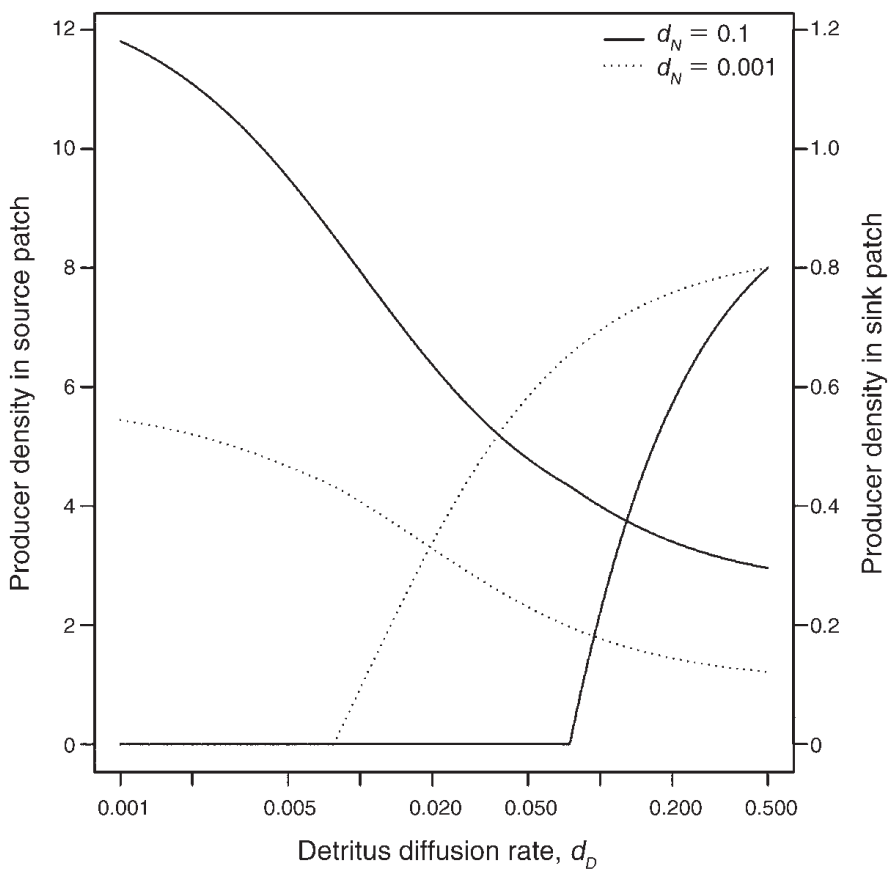
\includegraphics[height=0.7\textheight]{Figs/gravel2010c}\\
		\footnotesize Gravel et al. 2010. Ecology
	\end{center}

\end{frame}

%------------------------------
		
\begin{frame}{Food chain length}
	
	\begin{center}
		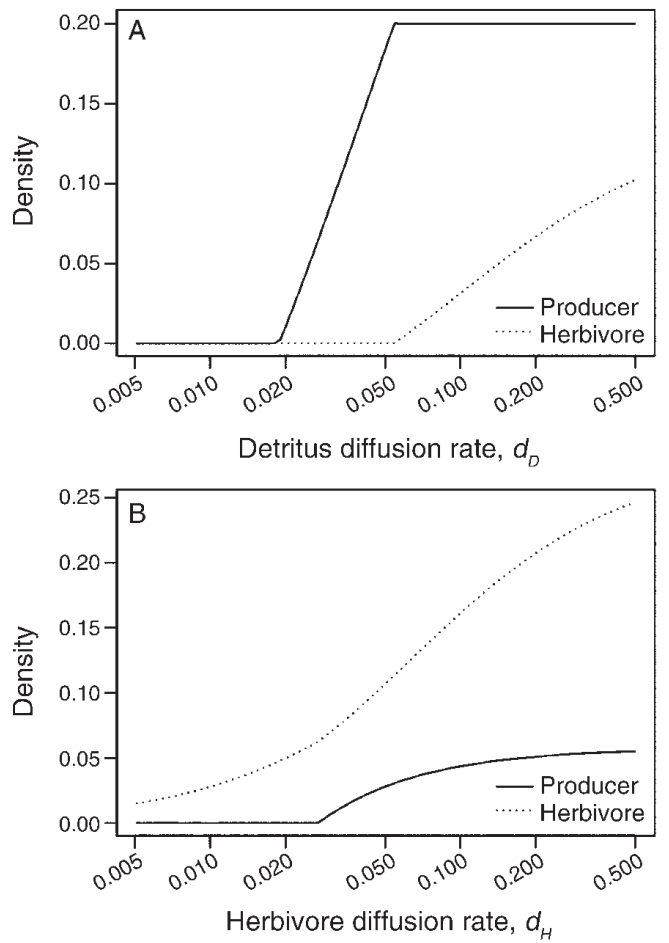
\includegraphics[height=0.7\textheight]{Figs/gravel2010d}\\
		\footnotesize Gravel et al. 2010. Ecology
	\end{center}

\end{frame}

%------------------------------
		
\begin{frame}{Paradox of enrichment}
	
	\begin{center}
		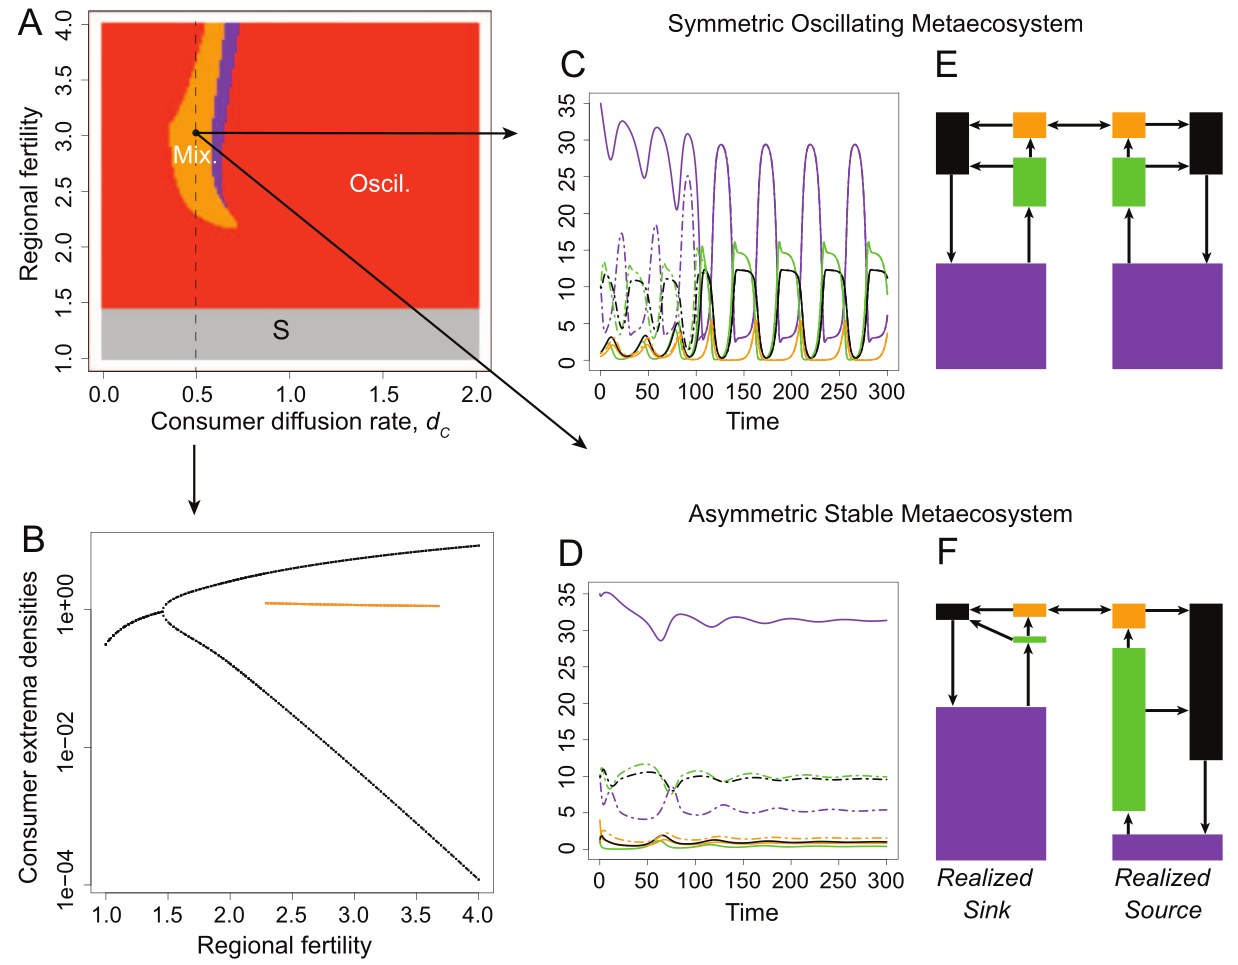
\includegraphics[height=0.7\textheight]{Figs/gounand2014}\\
		\footnotesize Gounand et al. 2014. Am. Nat.
	\end{center}

\end{frame}

%------------------------------
					
\begin{frame}{Source-sink dynamics}{Interpretations}
	
	\textbf{Demographic source/sink} : Habitat that is a net exporter/importer of individuals (Pulliam, 1988)

	\textbf{Fundamental source/sink} : Habitat in which a species’ density-independent growth rate is
	positive/negative in the absence of spatial flows (Gravel et al. 2010)

	\textbf{Realized source/sink} : Habitat in which a species’ density-independent growth rate is
	positive/negative in the presence of spatial flows (Gravel et al. 2010)

	\textbf{Conditional/Unconditional source/sink} : Subsystem that produces/absorbs a surplus of specific living or
	non-living entities under some/all conditions (Loreau et al. 2013)

\end{frame}

%------------------------------
% SPATIAL CASCADES
%------------------------------

{
	\usebackgroundtemplate{}
	\begin{frame}
	
		\pagecolor{BDQC1st}
		\color{white}
	
		\LARGE{\textit{Spatial cascades}}
	
	\end{frame}
}
		
%------------------------------
		
\begin{frame}{Trophic cascades}
	
	\begin{center}
		
\includegraphics[height=0.75\textheight]{Figs/estes2011}\\
		\footnotesize Estes et al. 2011. Science
	\end{center}

\end{frame}

%------------------------------
			
\begin{frame}{Indirect interactions in food webs}
	
	\begin{center}
		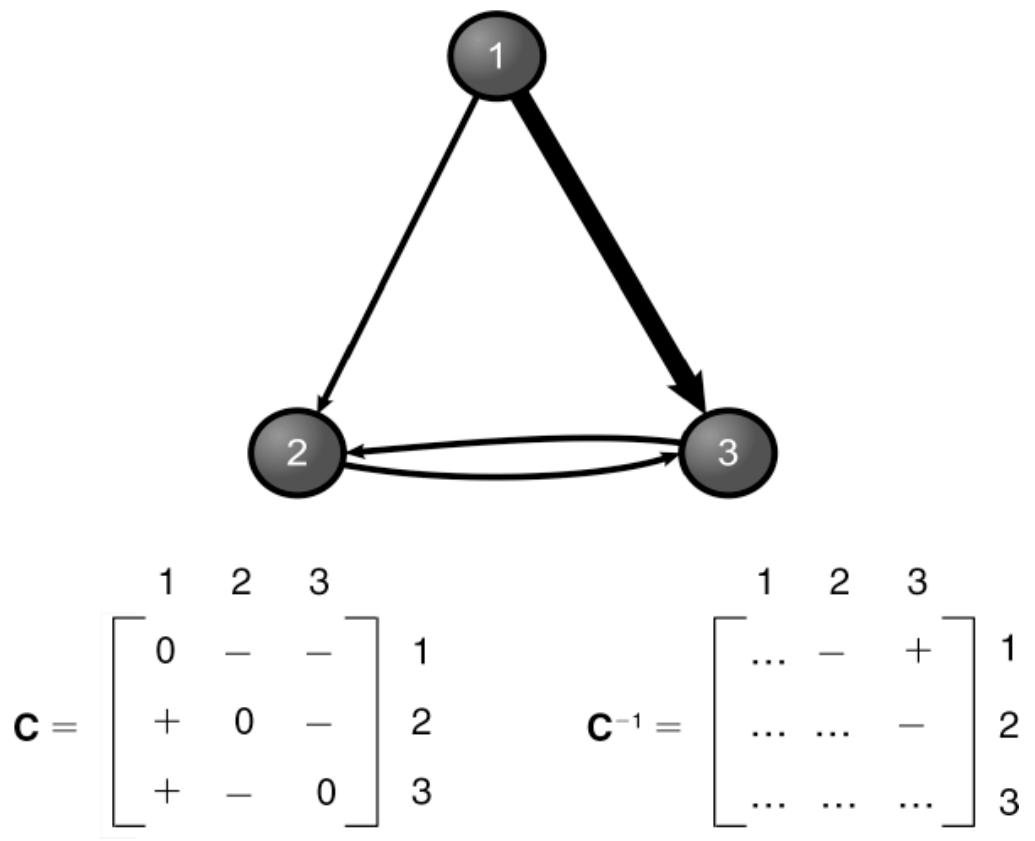
\includegraphics[height=0.7\textheight]{Figs/montoya2009a}\\
		\footnotesize Montoya et al. 2009. Ecology
	\end{center}

\end{frame}

%------------------------------
			
\begin{frame}{Indirect interactions in food webs}
	
	\begin{center}
		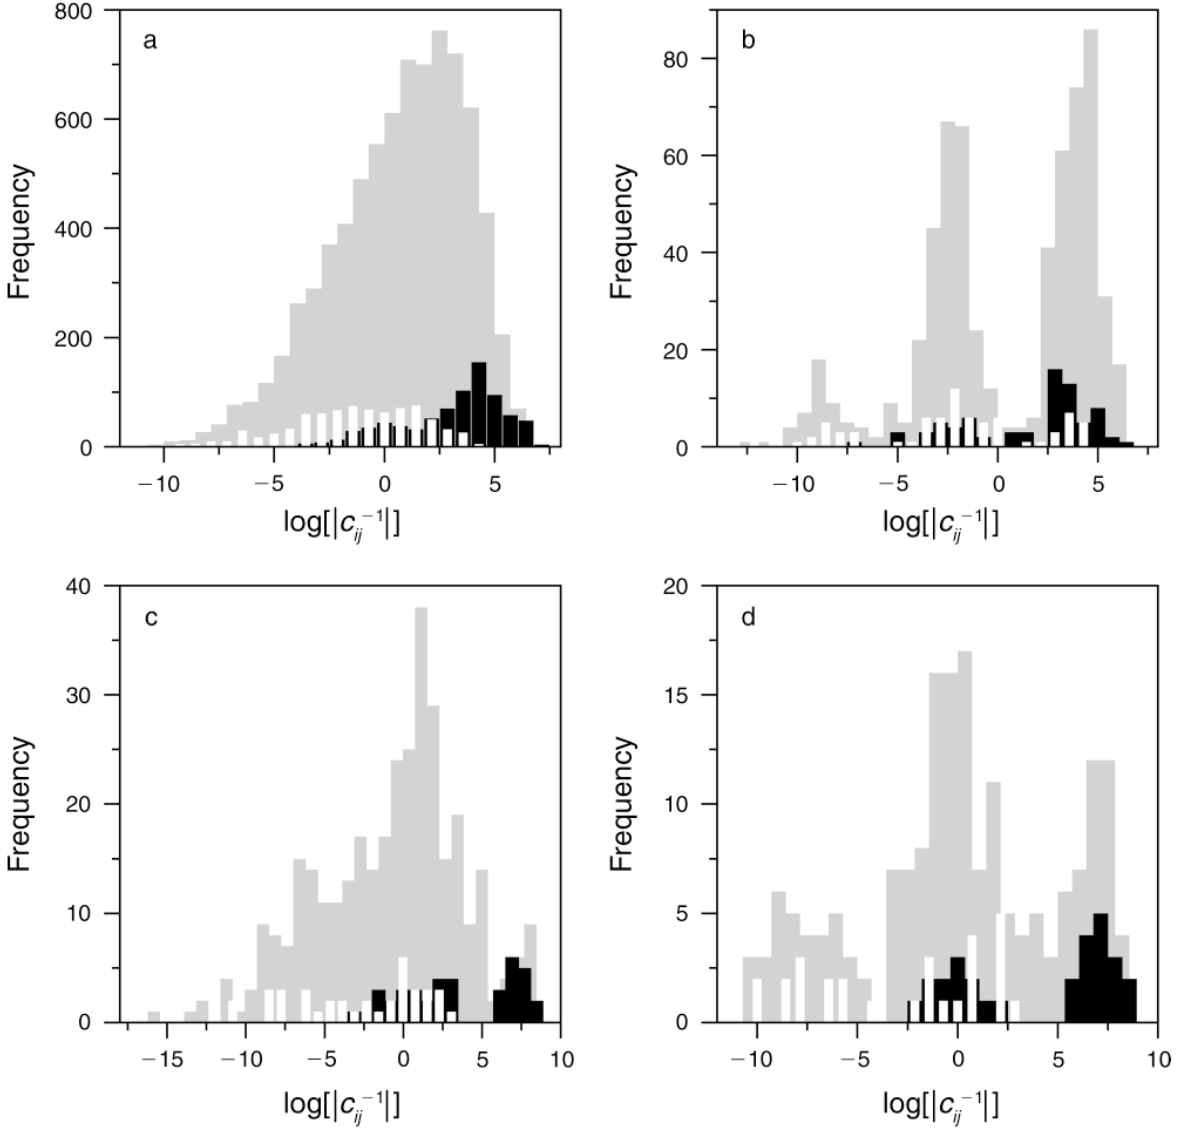
\includegraphics[height=0.7\textheight]{Figs/montoya2009b}\\
		\footnotesize Montoya et al. 2009. Ecology
	\end{center}

\end{frame}

%------------------------------
			
\begin{frame}{Indirect interactions in food webs}{Metaecosystems}
	
	\begin{center}
		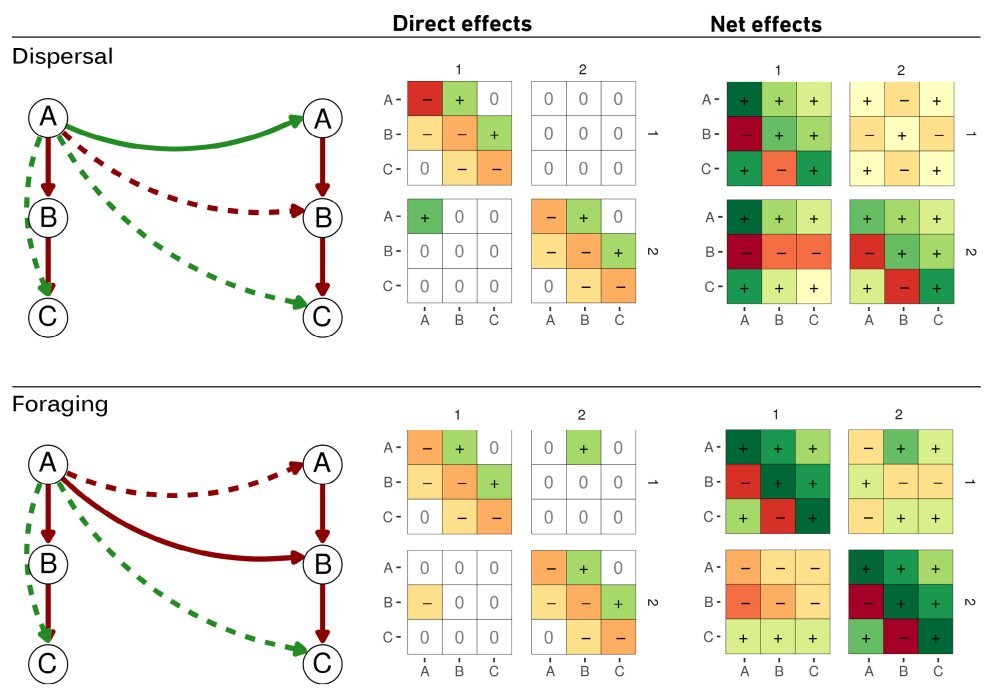
\includegraphics[height=0.7\textheight]{Figs/garcia2019a}\\
		\footnotesize Garcia et al. 2019. Ecology
	\end{center}

\end{frame}

%------------------------------					
					
\begin{frame}{Spatial cascades}{Model}
	
	\begin{center}
		
\includegraphics[height=0.7\textheight]{Figs/gravel2016a}\\
		\footnotesize Gravel et al. 2016. Nat. Communications
	\end{center}

\end{frame}

%------------------------------

\begin{frame}{Spatial cascades}{Emerging indirect interactions}
	
	\begin{center}
		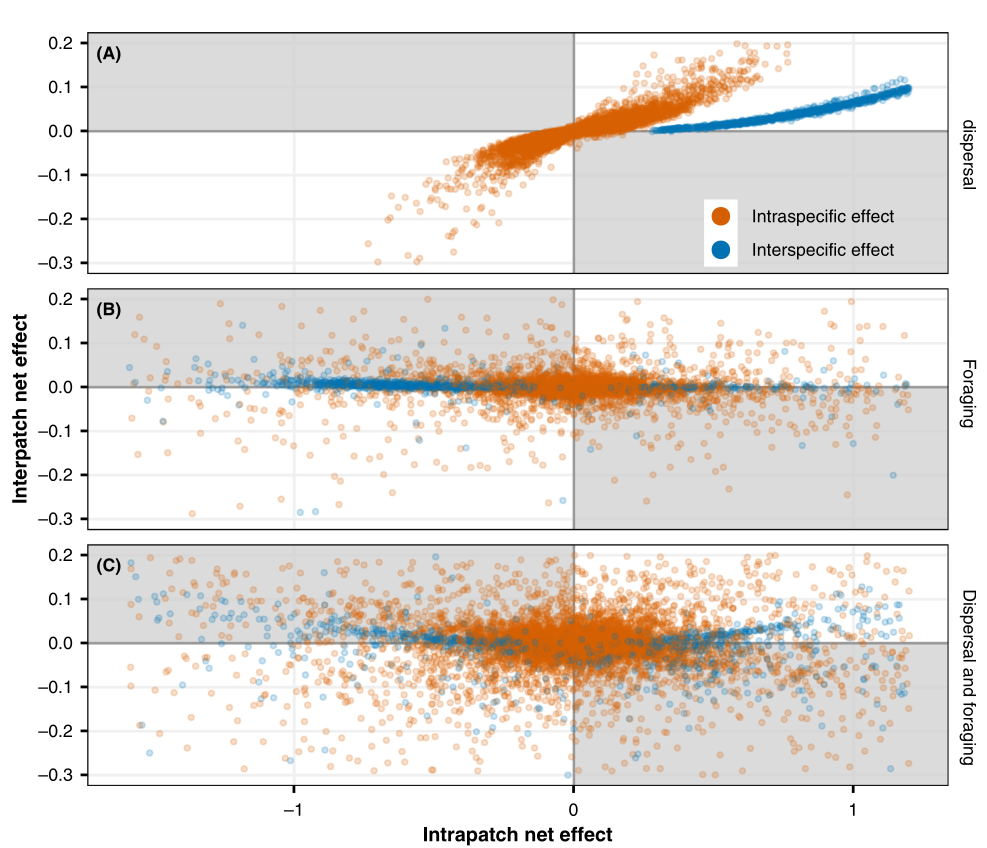
\includegraphics[height=0.7\textheight]{Figs/garcia2019b}\\
		\footnotesize Garcia et al. 2019. Ecology
	\end{center}

\end{frame}

%------------------------------					
			
\begin{frame}{Spatial cascades}{Spatial structure}
	
	\begin{center}
		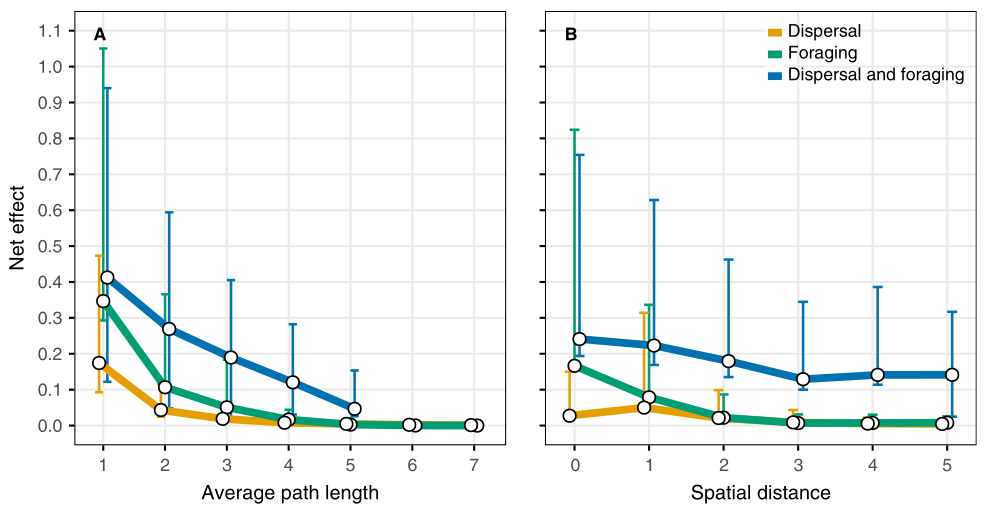
\includegraphics[height=0.7\textheight]{Figs/garcia2019c}\\
		\footnotesize Garcia et al. 2019. Ecology
	\end{center}

\end{frame}

%------------------------------					
			
\begin{frame}{Metaecosystem dynamics}{Conclusion}
	
	\begin{itemize}
		\item Local productivity may depend on surrounding ecological context
		\item Energy and nutrient flows may alter food web structure and dynamics
		\item Contingent source-sink dynamics spatial ecosystems
		\item Very conceptual, needs concrete application
	\end{itemize}

\end{frame}

%------------------------------
% MIGRATION
%------------------------------	

{
	\usebackgroundtemplate{}
	\begin{frame}
	
		\pagecolor{BDQC1st}
		\color{white}
	
		\LARGE{\textit{Migration as a unique spatial flow}}
	
	\end{frame}
}
		
%------------------------------
		
\begin{frame}{Actual theory}
	
	\begin{center}
		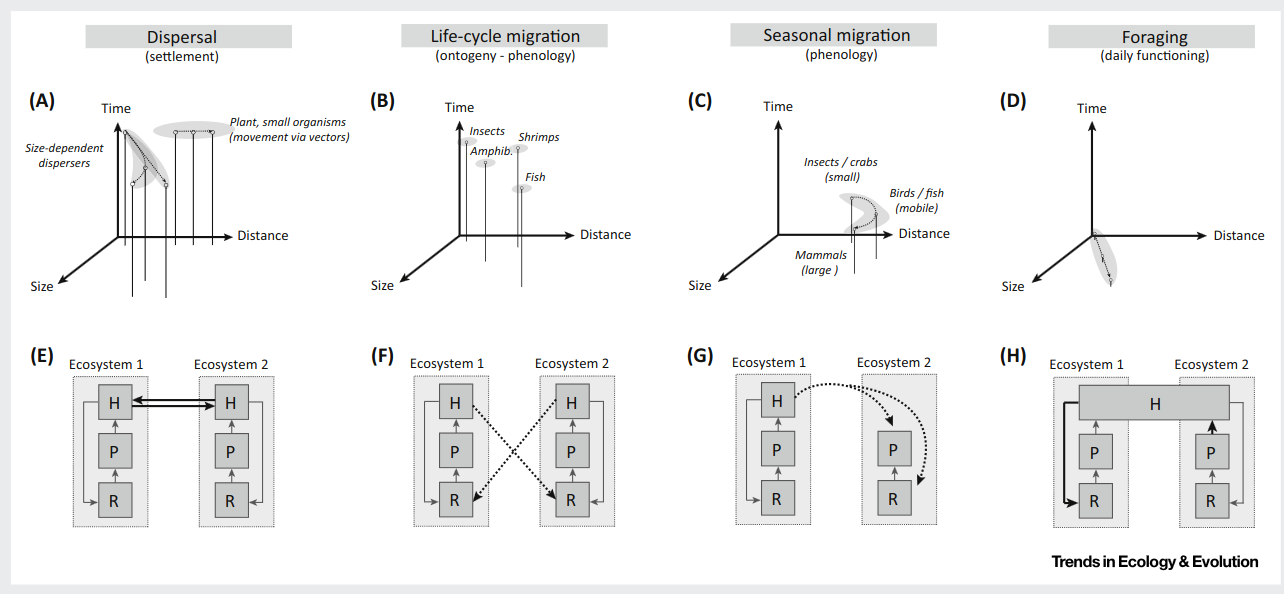
\includegraphics[height=0.6\textheight]{Figs/gounand2018}\\
		\footnotesize Gounand et al. 2018. TREE
	\end{center}

\end{frame}

%------------------------------	
		
\begin{frame}{Actual theory}
	
	\begin{center}
		
\includegraphics[height=0.7\textheight]{Figs/gravel2016a}\\
		\footnotesize Gravel et al. 2016. Nat. Communications
	\end{center}

\end{frame}

%------------------------------	
				
\begin{frame}{Unique features of migration}
	
	\begin{itemize}
		\item Happens at very specific moment of the year
		\item High frequency and repeated
		\item Include all individuals
		\item Very short 
		\item Very species-specific
	\end{itemize}

\end{frame}

%------------------------------	

\begin{frame}{Migration networks}
	\begin{center}
		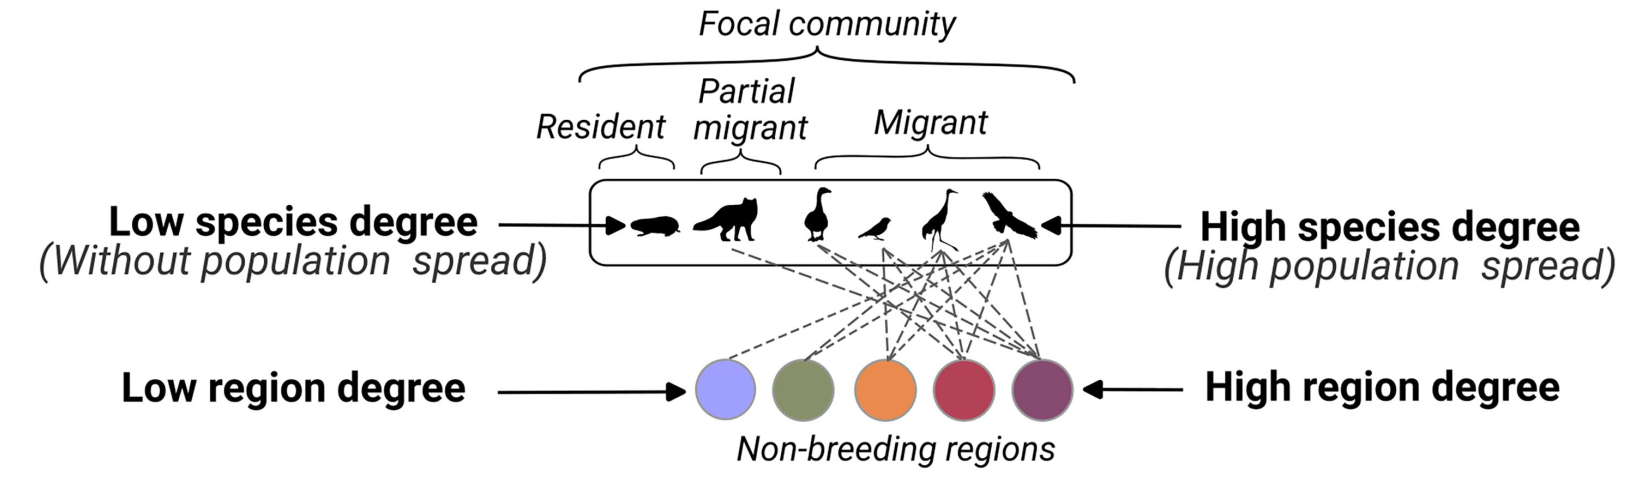
\includegraphics[height=0.4\textheight]{Figs/moisan2022a}\\
		\footnotesize{Moisan et al. 2022 \textit{Front. Ecol. Evol.}}
	\end{center}
\end{frame}

%------------------------------

\begin{frame}{Migration networks}
	\begin{center}
		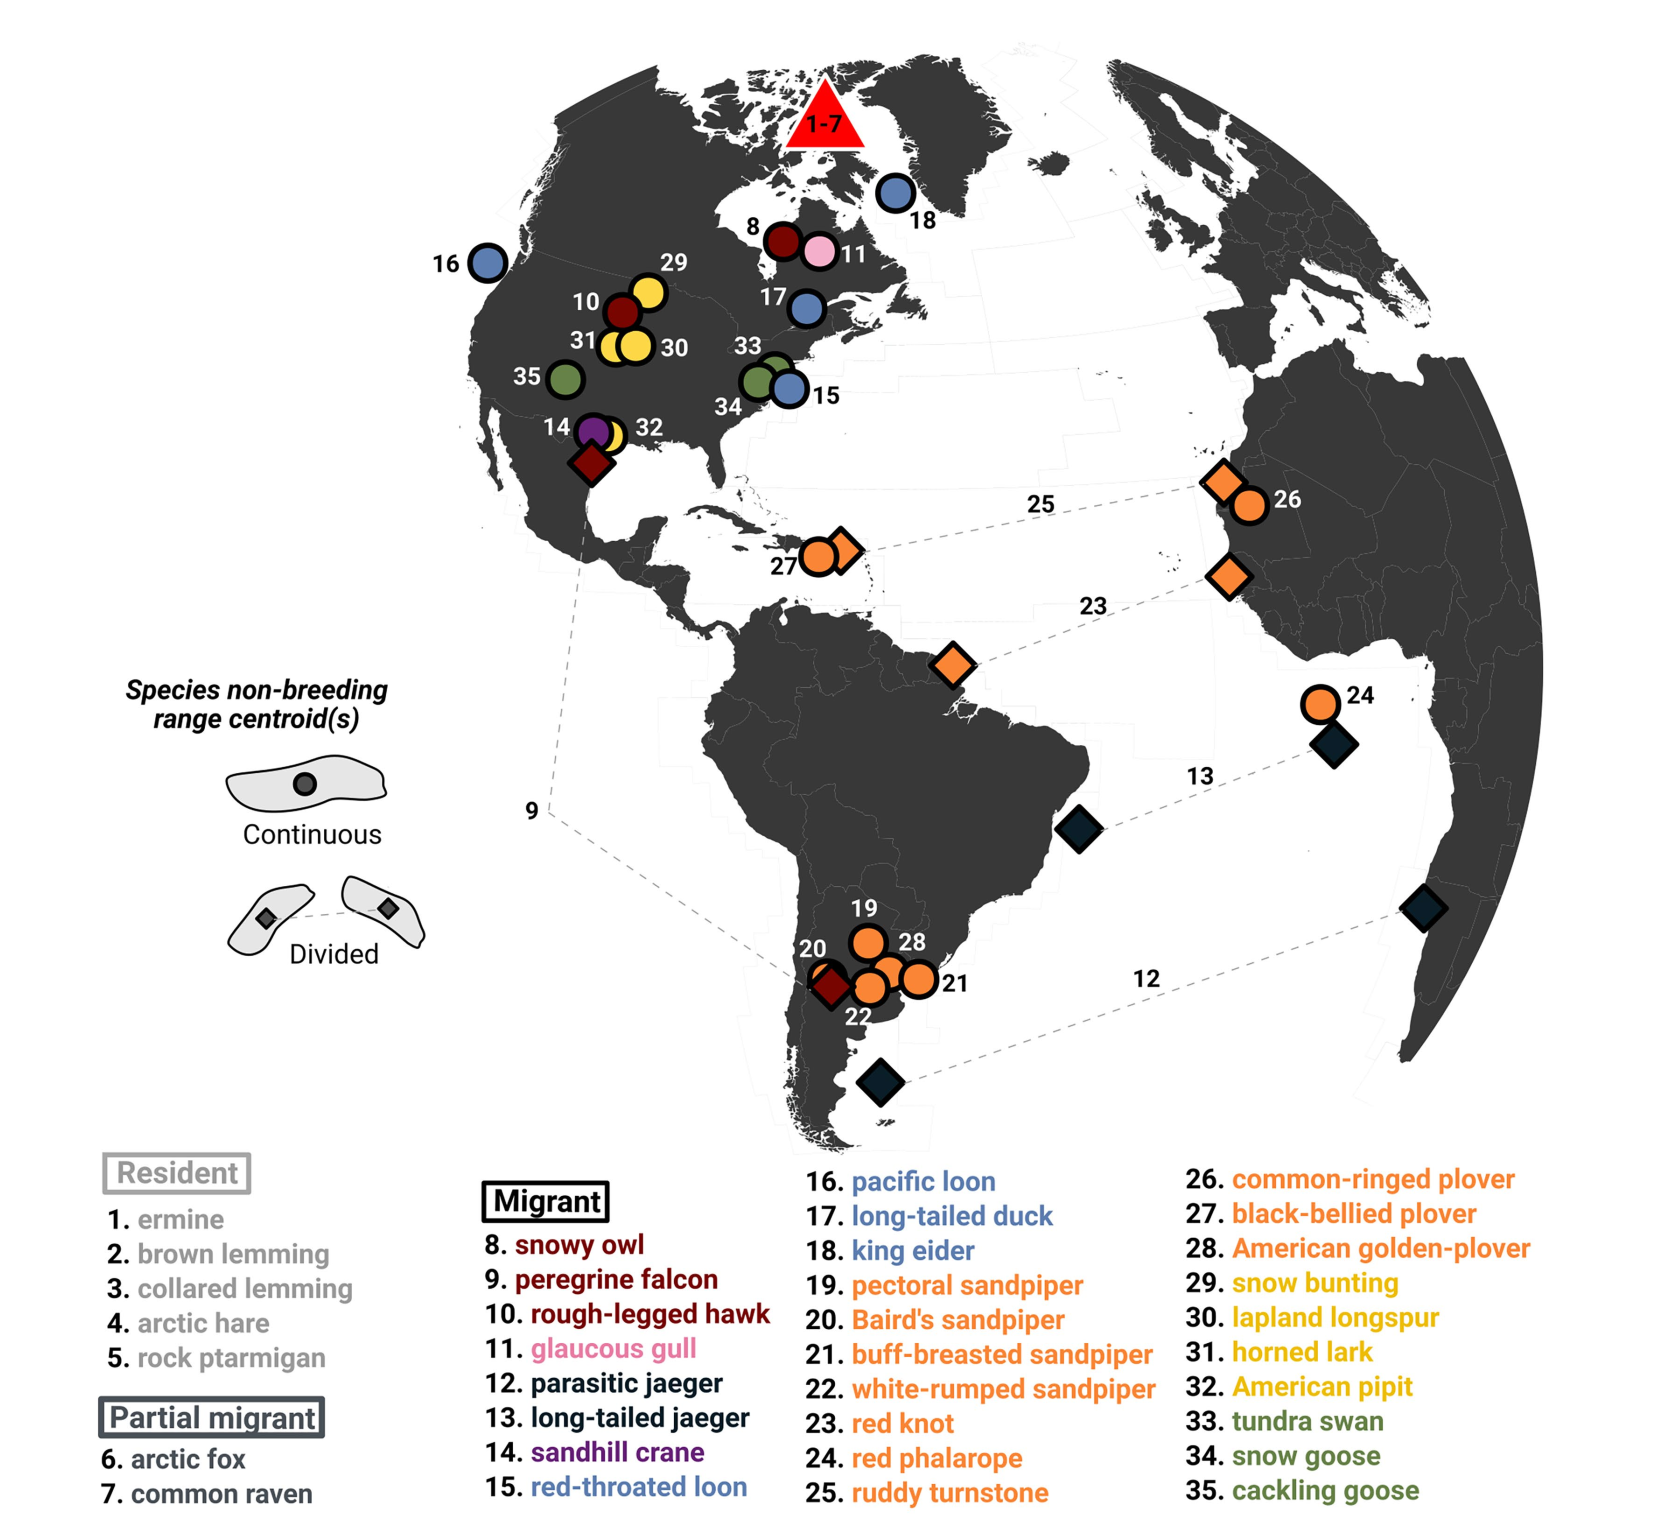
\includegraphics[height=0.75\textheight]{Figs/moisan2022b}\\
		\footnotesize{Moisan et al. 2022 \textit{Front. Ecol. Evol.}}
	\end{center}
\end{frame}

%------------------------------

\begin{frame}{Migration networks}
	\begin{center}
		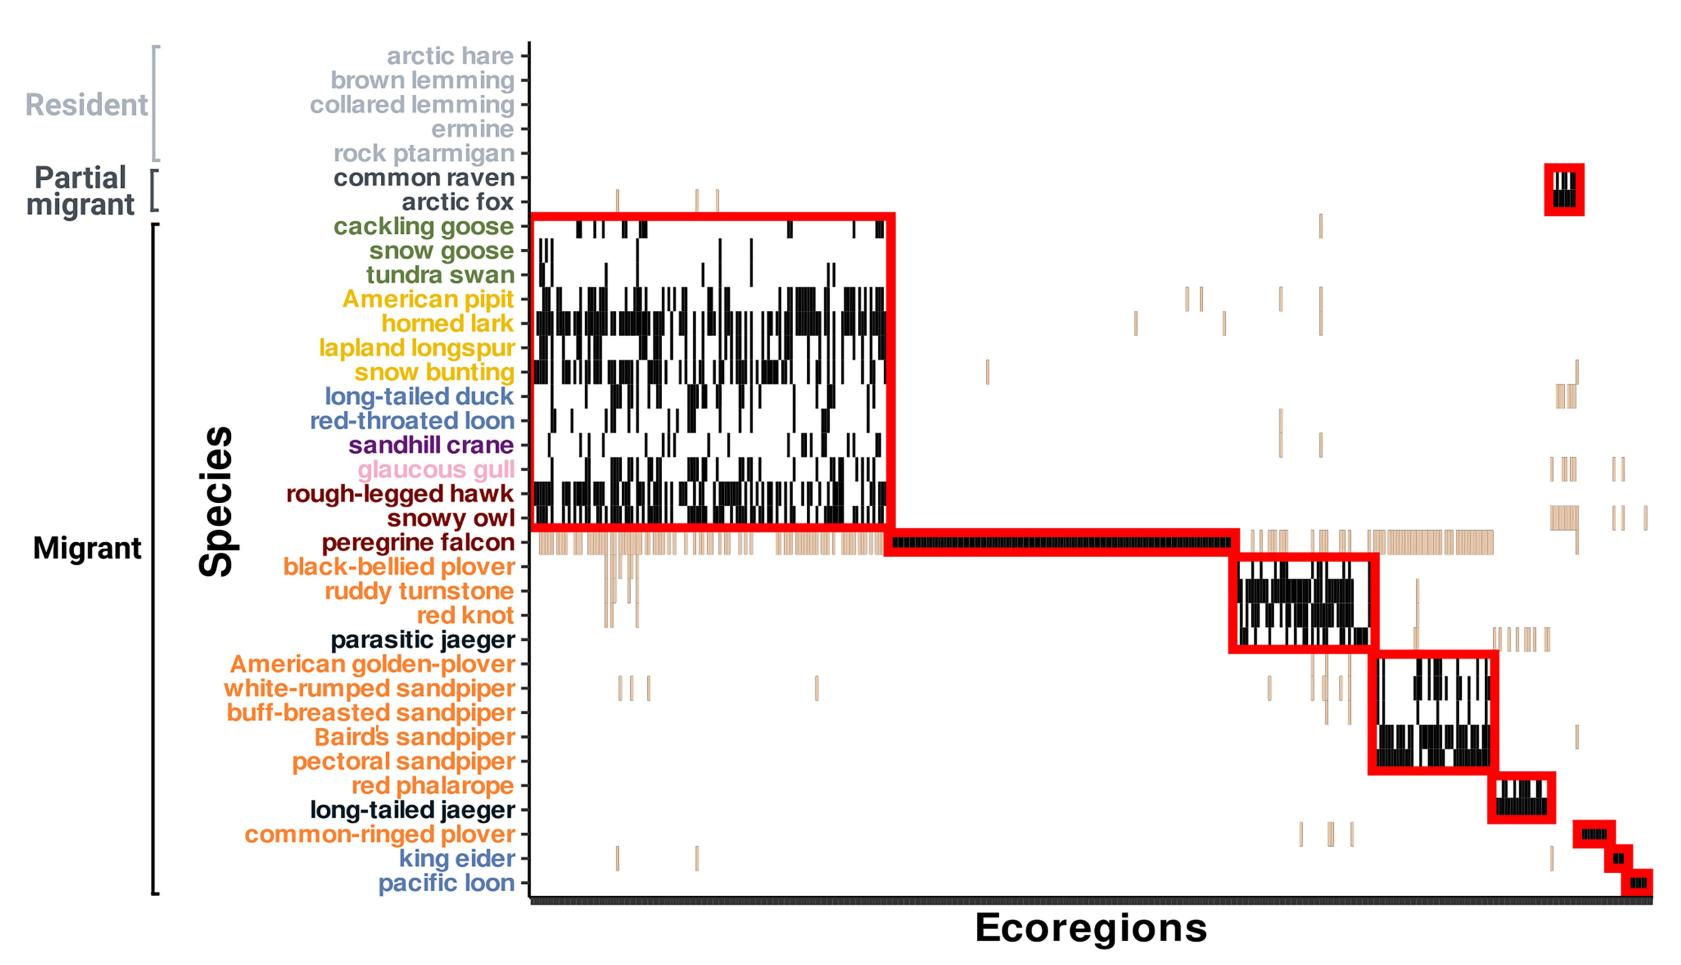
\includegraphics[height=0.75\textheight]{Figs/moisan2022c}\\
		\footnotesize{Moisan et al. 2022 \textit{Front. Ecol. Evol.}}
	\end{center}
\end{frame}

%------------------------------

\begin{frame}{Hybrid models}
	
	\begin{center}
		
\includegraphics[height=0.7\textheight]{Figs/hutchison2020}\\
		\footnotesize Hutchison et al. 2020. Phil. Trans. Roy. Soc. A
	\end{center}

\end{frame}

%------------------------------	
				
\begin{frame}{Hybrid models}{Stability}
	
	\begin{center}
		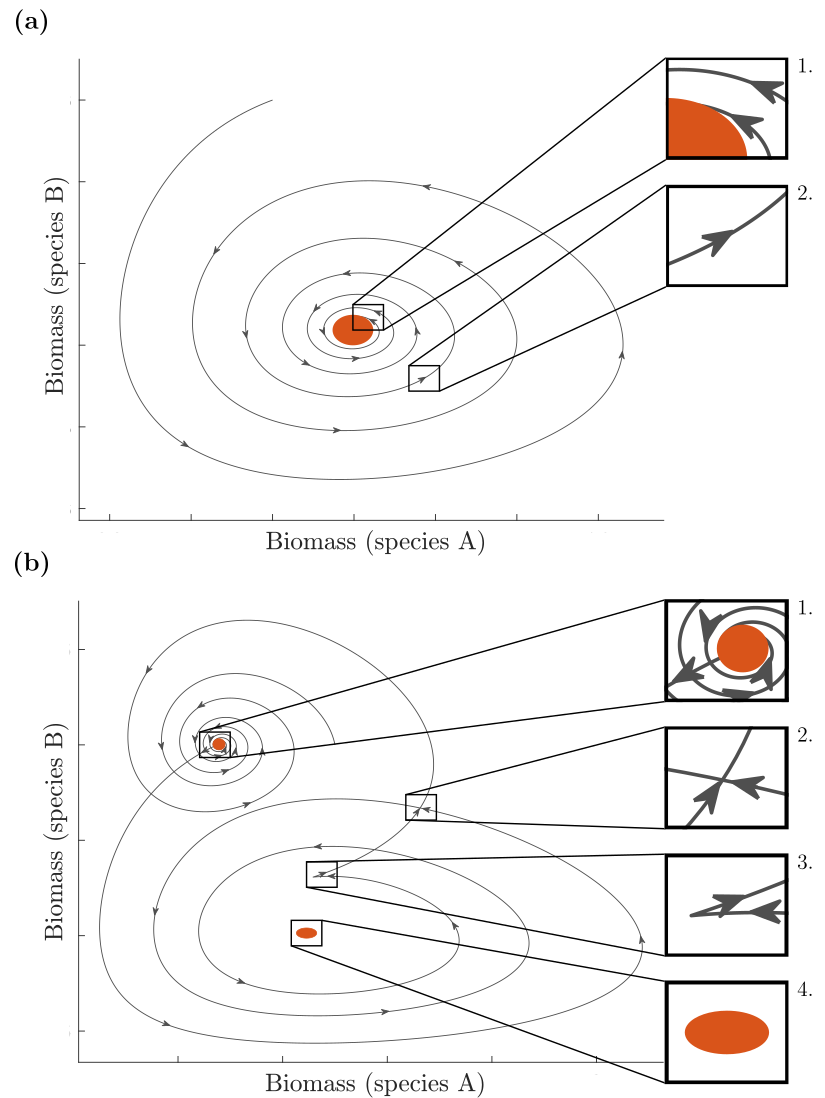
\includegraphics[height=0.7\textheight]{Figs/hutchison2024}\\
		\footnotesize Hutchison et al. 2024. Theoretical Ecology
	\end{center}

\end{frame}

%------------------------------	

\begin{frame}{State-dependent switches}
	\begin{center}
		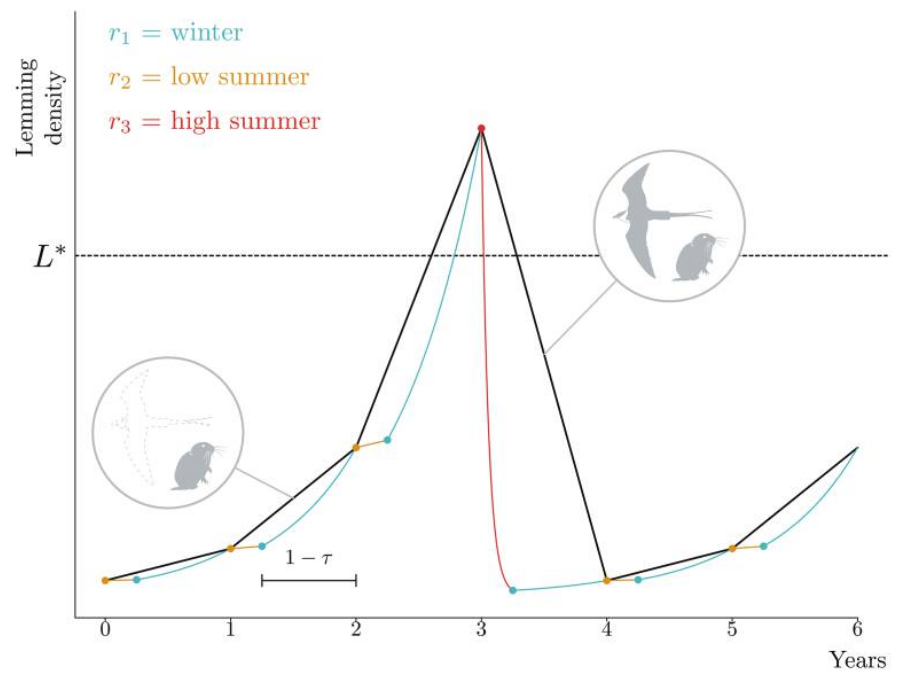
\includegraphics[height=0.6\textheight]{Figs/bergeron2026a}\\
		\footnotesize{Bergeron et al. 2026. Am. Nat}
	\end{center}
\end{frame}

%------------------------------

\begin{frame}{Stability revisited}
	\begin{center}
		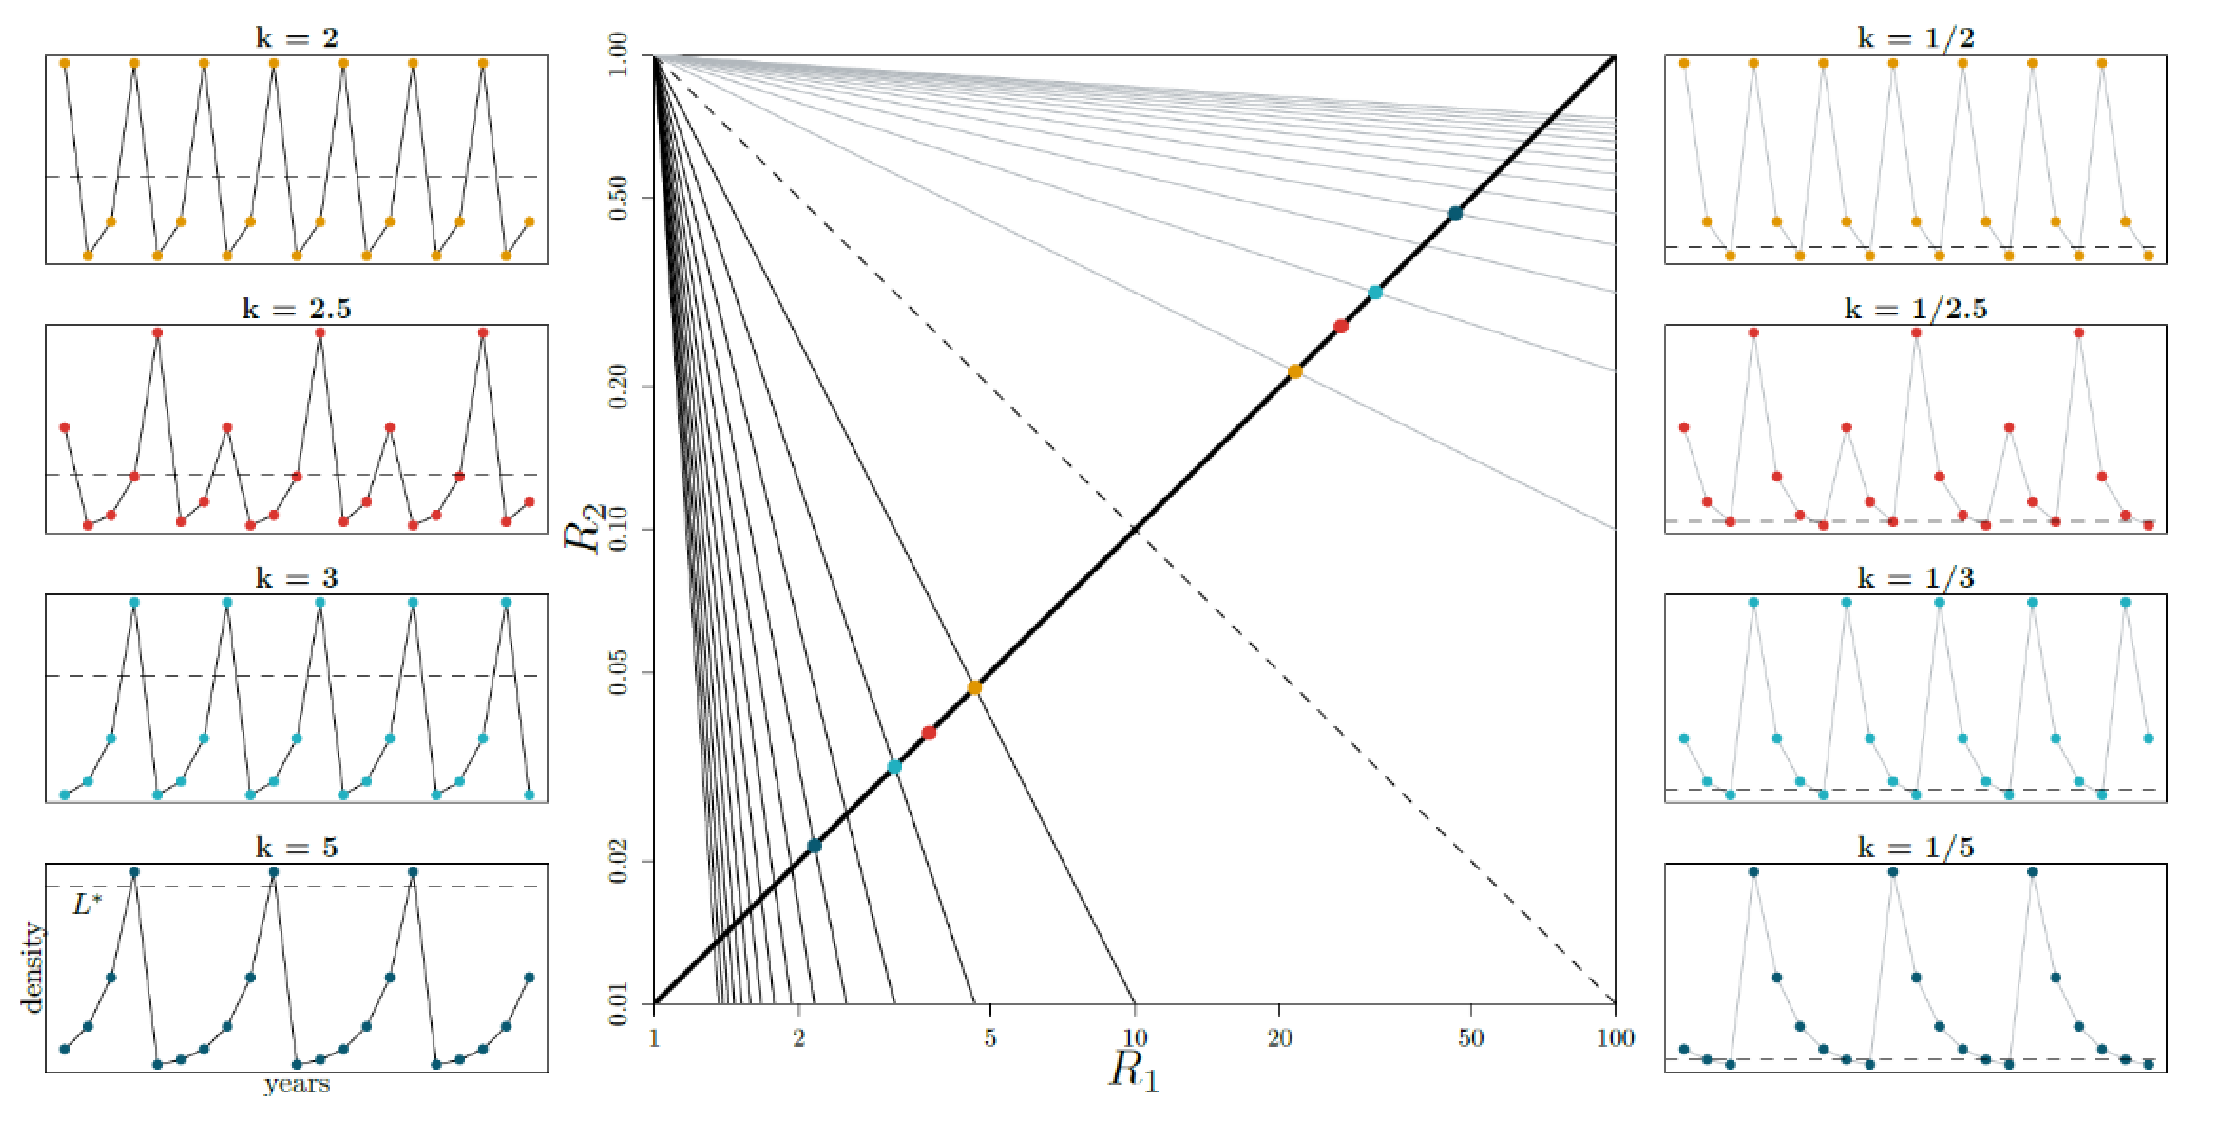
\includegraphics[height=0.6\textheight]{Figs/bergeron2026b}\\
		\footnotesize{Bergeron et al. 2026. Am. Nat}
	\end{center}
\end{frame}

%------------------------------

\begin{frame}{Application to lemming cycles}
	\begin{center}
		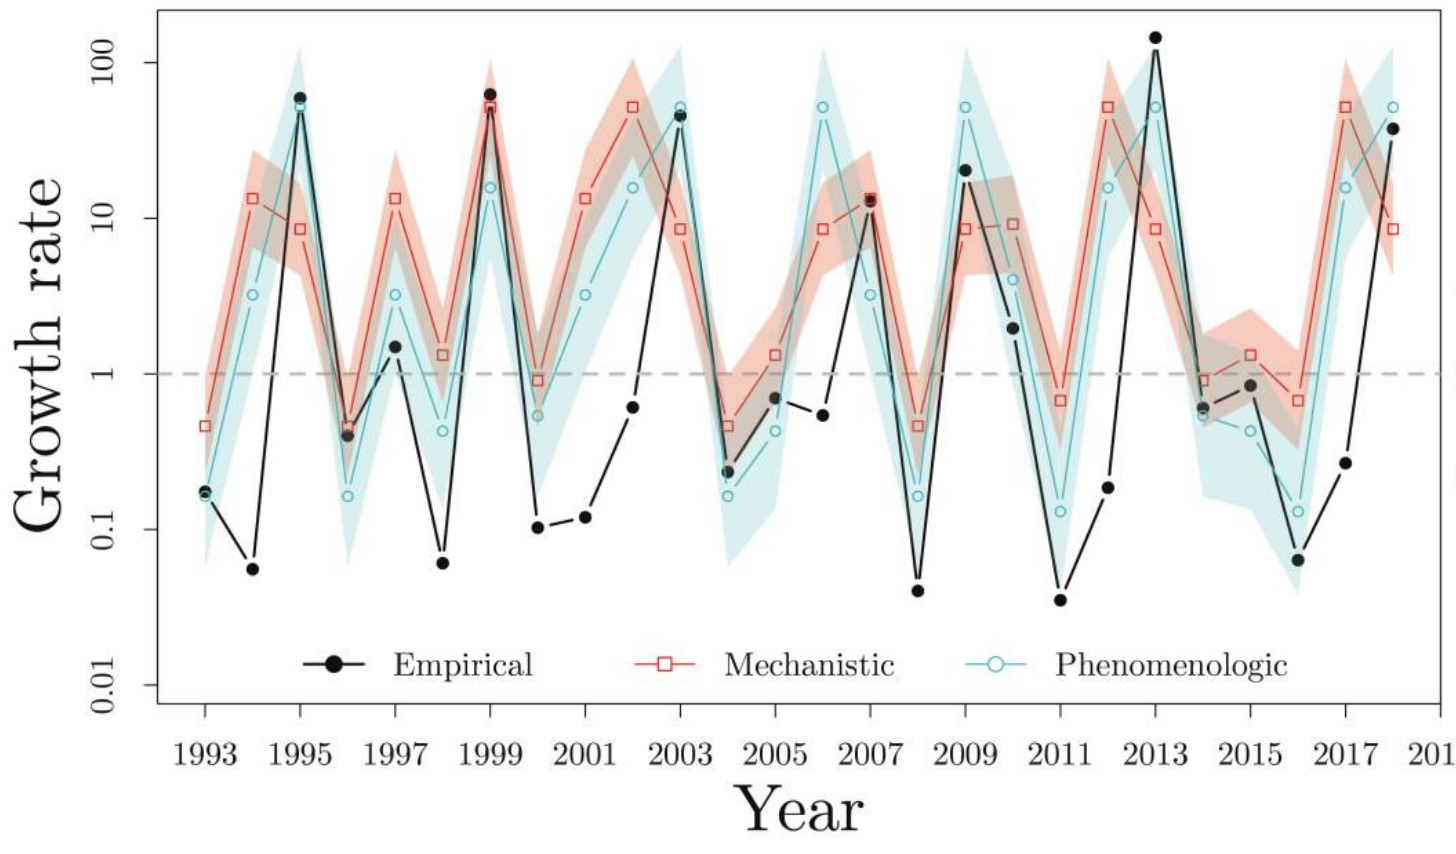
\includegraphics[height=0.75\textheight]{Figs/bergeron2026c}\\
		\footnotesize{Bergeron et al. 2026. Am. Nat}
	\end{center}
\end{frame}

%------------------------------																														

\begin{frame}{Open questions}
	\begin{itemize}
		\item What are appropriate metrics to describe and understand such networks ?
		\item How disturbances are spreading on such high dimensional networks ?
		\item How to track indirect interactions ?
	\end{itemize}
\end{frame}

%------------------------------
%------------------------------
%------------------------------
\end{document}
